% ---------------------------------------------------
% ----- Main document of the template
% ----- for Bachelor-, Master thesis and class papers
% ---------------------------------------------------
%  Created by Claudia Müller-Birn on 2012-08-17. (updated on 2013-04-03)
%  Freie Universität Berlin, Institute of Computer Science, Human Centered Computing (HCC). 
%
\documentclass[pdftex,a4paper,12pt]{scrartcl}   
%
%---------------------------------------------------
%----- Packages
%---------------------------------------------------
%
\usepackage[T1]{fontenc} 
\usepackage[utf8]{inputenc}
\usepackage[ngerman]{babel} %\usepackage[english]{babel}  
\usepackage{ae} 
\usepackage{bibgerm}    

\usepackage{fancyref} 
\usepackage{fancyhdr} % Define simple headings 
\usepackage{xcolor}
\usepackage{url}
%
\usepackage[pdftex]{graphicx}  
\usepackage{hyperref} % turn all your internal references into hyperlinks
%\usepackage[pdfstartview=FitH,pdftitle={<<Titel der Arbeit>>}, pdfauthor={<<Autor>>}, pdfkeywords={<<Schlüsselwörter>>}, pdfsubject={<<Titel der Arbeit>>}, colorlinks=true, linkcolor=black, citecolor=black, urlcolor=black, hypertexnames=false, bookmarksnumbered=true, bookmarksopen=true, pdfborder = {0 0 0}]{hyperref}
% 
% a new command is defined that allows to include an empty page when needed
\newcommand{\blankpage}{
\newpage
\thispagestyle{empty}
\mbox{}
\newpage
}
%
%---------------------------------------------------
%----- PDF and document setup
%---------------------------------------------------
%
\hypersetup{
	pdftitle={<My title>},  % please, add the title of your thesis
    pdfauthor={<Author>},   % please, add your name
    pdfsubject={<<Bachelor thesis>, Institute of Computer Science, Freie Universität Berlin>}, % please, select the type of this document
    pdfstartview={FitH},    % fits the width of the page to the window
    pdfnewwindow=true, 		% links in new window
    colorlinks=false,  		% false: boxed links; true: colored links
    linkcolor=red,          % color of internal links
    citecolor=green,        % color of links to bibliography
    filecolor=magenta,      % color of file links
    urlcolor=cyan           % color of external links
}
%
%---------------------------------------------------      
%----- Settings for word separation  
%---------------------------------------------------      
% Help for separation (from package babel, section 22)):
% In german package the following hints are additionally available:
% "- = an explicit hyphen sign, allowing hyphenation in the rest of the word
% "| = disable ligature at this position. (e.g., Schaf"|fell)
% "~ = for a compound word mark without a breakpoint (e.g., bergauf und "~ab)
% "= = for a compound word mark with a breakpoint, allowing hyphenation in the composing words
% "" = like "-, but producing no hyphen sign (e.g., und/""oder)
%
% Describe separation hints here:
\hyphenation{
% Pro-to-koll-in-stan-zen
% Ma-na-ge-ment  Netz-werk-ele-men-ten
% Netz-werk Netz-werk-re-ser-vie-rung
% Netz-werk-adap-ter Fein-ju-stier-ung
% Da-ten-strom-spe-zi-fi-ka-tion Pa-ket-rumpf
% Kon-troll-in-stanz
}

%---------------------------------------------------      
%----- Settings for title page 
%---------------------------------------------------

\begin{titlepage}

\title{
{\small <Bachelorarbeit> am Institut für Informatik der Freien Universität Berlin}\\
{\small Human-Centered Computing (HCC), AG NBI}\\
[6ex]
{\LARGE<Titel der Arbeit>}\\
{\normalsize-- Exposé --}}

\author{
{\emph{\normalsize<Ihr Vor- und Nachname>}}\\
{\normalsize Matrikelnummer: <IhreMatrikelnummer>}\\
{\normalsize <ihreemail@adresse.de>}\\\\
{\normalsize Betreuerin: Prof. Dr. C. Müller-Birn}
}

\date{\normalsize Berlin, <Datum>}

\end{titlepage}

%%%%%%%%%%%%%%%%%%%%%%%%%%%%%%%%%%%%%%%%%%%%%%%%%%%%%%
% The content part of the documentent starts here! %%
%%%%%%%%%%%%%%%%%%%%%%%%%%%%%%%%%%%%%%%%%%%%%%%%%%%%%%

\begin{document}

\maketitle 

\thispagestyle{empty}  % eliminate page number on the title page

\blankpage

%---------------------------------------------------      
%----- Content part  
%---------------------------------------------------

\setcounter{page}{1} % page number is set to "1" otherwise it would be "3"

\section{Struktur des Exposé}
Im Folgenden habe ich Ihnen eine generelle Struktur für ein Exposé vorgegeben. Jeder Abschnitt ist mit einer Frage, welchen Inhalt dieses Kapitel abdecken sollte eingeleitet und enthält einige Erläuterungen. Bitte beachten Sie, dass das Layout dieser Vorlage doppelseitig angelegt ist.

\subsection{Motivation der Arbeit} 
\begin{itemize}
	\item In welchem Bereich/Themenfeld bewegt sich Ihre geplante Arbeit?
	\item Erläutern Sie kurz, in welchem Themenbereich Ihre Arbeit angesiedelt ist. Wo werden Sie einen Beitrag leisten?
	\item Nutzen Sie bei den Erläuterungen die Ihnen bereitgestellte Kurzaufgabenstellung.
\end{itemize} 

\subsection{Thematische Einordnung der Arbeit}
\begin{itemize}
	\item Welche Artikel/Literatur sind/ist relevant für diese Arbeit? 
	\item Bitte geben Sie die relevanten Inhalte der Artikel kurz wieder.
	\item Das Ausarbeiten von ausgewählter Literatur bzw. verwandten Arbeiten hilft Ihnen, Ihre Ziele im folgenden Abschnitt zu definieren. Daher ist eine Auseinandersetzung mit der Literatur von Beginn an notwendig, wenn es zu diesem Zeitpunkt noch nicht erschöpfend sein muss.
\end{itemize}

\subsection{Zielstellung} 
\begin{itemize}
	\item Welche Ziele werden mit der Arbeit verfolgt? Und welche zentralen Fragen lassen sich daraus ableiten?
	\item Die Ziele sollten so spezifisch wie möglich sein. Das hilft Ihnen im Verlauf der Umsetzung zu prüfen, ob Sie Ihre Ziele erreichen konnten.
\end{itemize}

\subsection{Geplante Vorgehensweise}
\begin{itemize}
	\item Welche einzelnen Aktivitäten müssen umgesetzt werden, um die Fragen zu beantworten und das Ziel der Arbeit zu erreichen?
	\item Aus den Fragen (vorheriger Abschnitt) können Sie dann gut Aktivitäten ableiten, die Ihnen helfen, Ihre weitere Arbeit zu strukturieren.
\end{itemize}

\subsection{Technische Umsetzung}
\begin{itemize}
	\item Mit welchen softwaretechnischen Hilfsmitteln soll die Arbeit realisiert werden?
	\item Selbstverständlich können Sie an der Stelle noch nicht alles wissen, aber Sie sollen sich hier bereits einen guten Überblick verschaffen.
\end{itemize}

\subsection{Erster Terminplan}
\begin{itemize}
	\item Wie ist der generelle Zeitplan der Arbeit? 
	\item Sie sollten bereits wissen, wann Sie fertig sein wollen und von dort mit der Rückwärtsterminierung starten.
	\item Ihre Arbeit ist ein Projekt, daher planen Sie es auch wie eines. Nutzen Sie zur Visualisierung ein Gantt-Chart.
\end{itemize}

\section{Wie geht es nach dem Exposé weiter?}

Nachdem die Phase der Exposé-Erstellung abgeschlossen ist (das kann bis zu drei Iterationen dauern), können Sie mit der Erstellung der eigentlichen Abschlussarbeit beginnen. Bitte nutzen Sie die Inhalte des Exposés gleich als inhaltlichen Rahmen für die Arbeit (vor allem in Kapitel 1). Ihnen wird wieder eine \LaTeX Vorlage zur Verfügung gestellt. In dieser Vorlage finden Sie wieder viele Informationen und Hilfestellungen zur Erstellung der Arbeit. Sie sollten nun Ihre Arbeit anmelden. Das entsprechende Formular finden Sie auf den Institutsseiten (\href{http://www.mi.fu-berlin.de/inf/stud-bioinf/downloads/Anmeldung_zur_Bachelorarbeit_2010.pdf}{Link}).Bitte bringen Sie das ausgefüllte Formular zu einer unserer Sitzungen mit. Ich unterschreibe es und leite es weiter. Nun sollten Sie auch bald darüber nachdenken, wer der Zweitgutachter Ihrer Arbeit sein könnte. Ich berate Sie dabei gern. 

Viele weitere, nützliche Informationen finden Sie in der Prüfungsordnung Ihres Studiengangs. Bitte lesen Sie den Sie betreffenden Absatz im Anhang (\ref{sec:bachelor}). 
%---------------------------------------------------
%----- Bibliography
%---------------------------------------------------
\newpage
\phantomsection
\addcontentsline{toc}{chapter}{Literatur}   % headline
\bibliographystyle{alpha}  % citation style
\bibliography{references} % bib file

\newpage 
\section*{Anhang I: Auszug Prüfungsordnung Bachelor}
\label{sec:bachelor}     
\begin{figure}[!h]
	\centering
		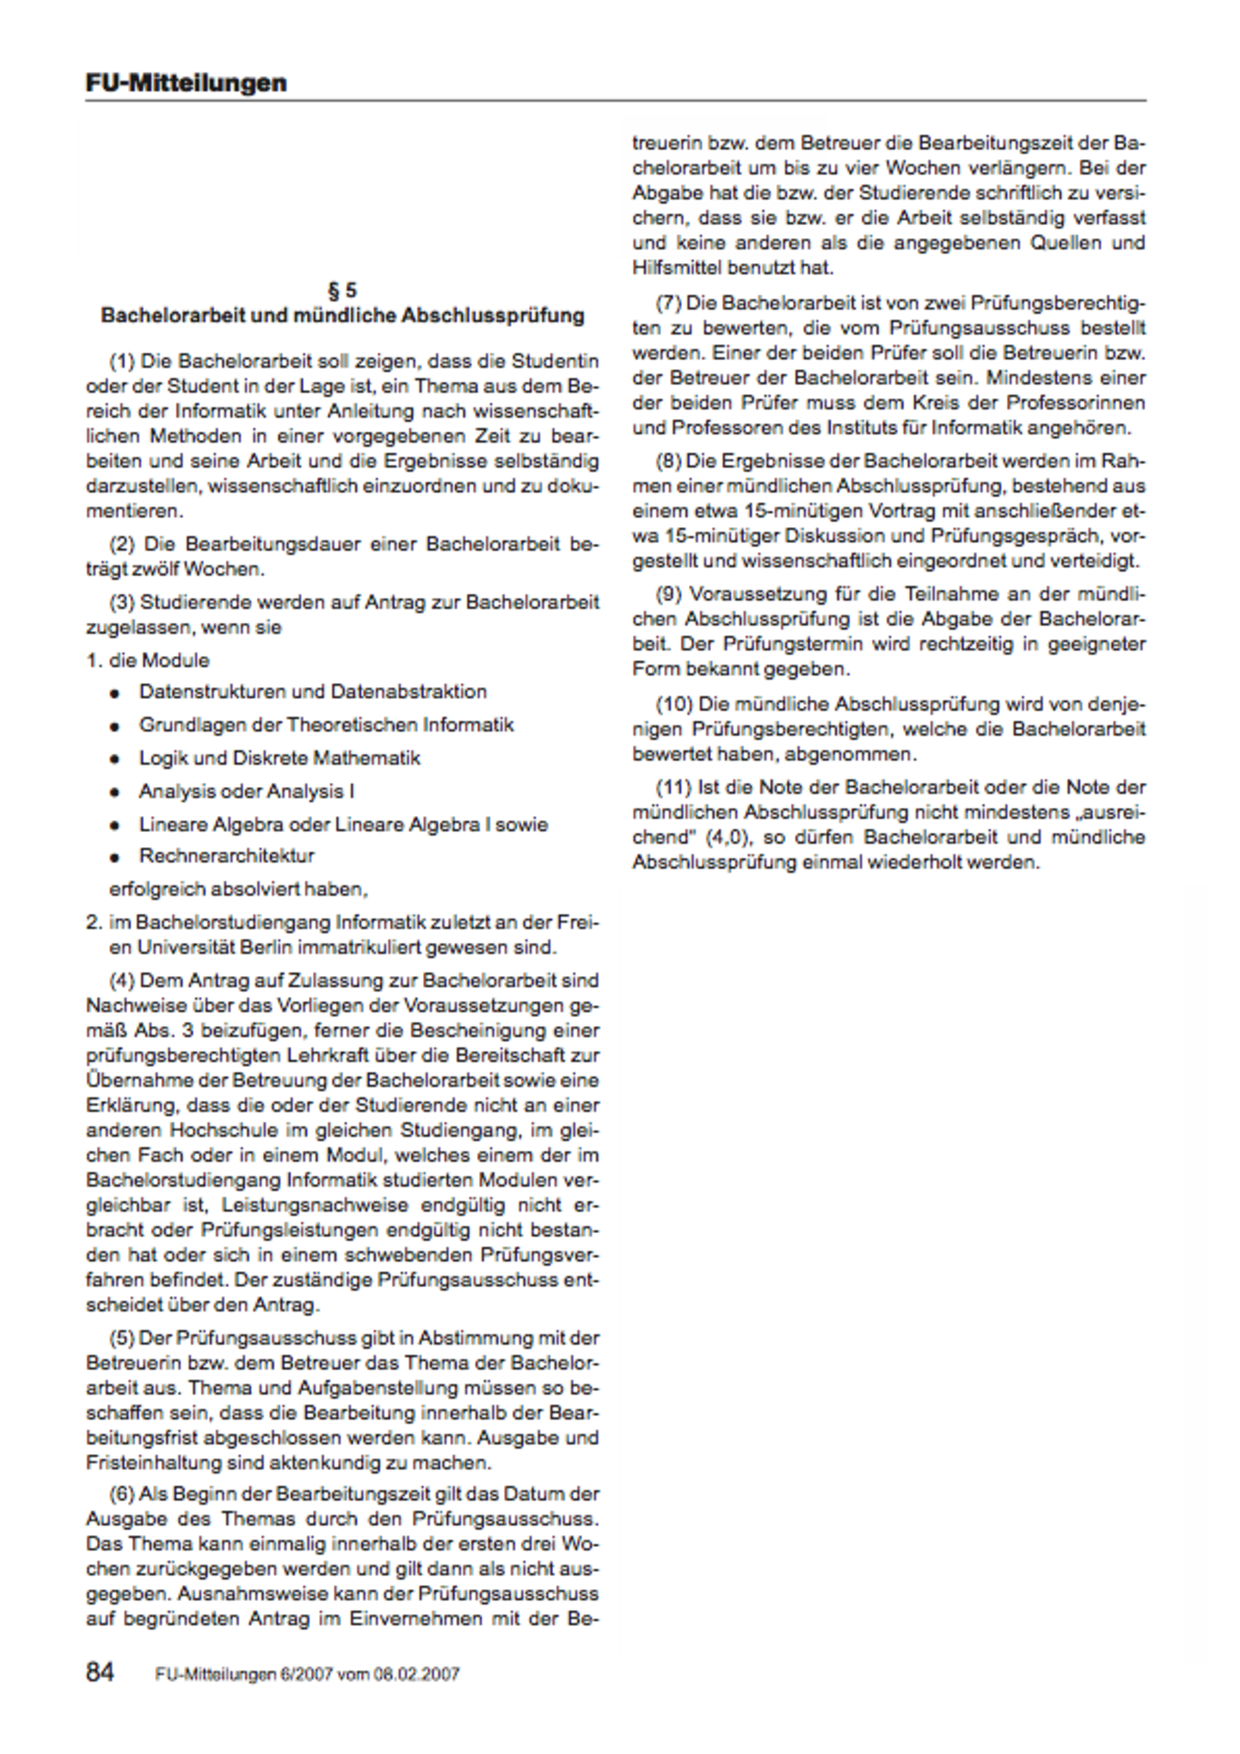
\includegraphics[width=0.8\textwidth]{../../img/proposal/Auszug_Bachelor_Pruefungsordnung.pdf}
	\caption{Auszug Prüfungsordnung Bachelor} 
\end{figure}

\end{document}